\let\negmedspace\undefined
\let\negthickspace\undefined
\documentclass[journal,12pt,onecolumn]{IEEEtran}
\usepackage{cite}
\usepackage{amsmath,amssymb,amsfonts,amsthm}
\usepackage{algorithmic}
\usepackage{graphicx}
\graphicspath{{./figs/}}
\usepackage{textcomp}
\usepackage{xcolor}
\usepackage{txfonts}
\usepackage{listings}
\usepackage{enumitem}
\usepackage{mathtools}
\usepackage{gensymb}
\usepackage{comment}
\usepackage{caption}
\usepackage[breaklinks=true]{hyperref}
\usepackage{tkz-euclide} 
\usepackage{listings}
\usepackage{gvv}    
\usepackage{multicol}




\begin{document}
\title{
ASSIGNMENT 5: GATE 2024\\
GG : Geology and Geophysics}
\author{EE25BTECH11003 -Adharvan Kshathriya Bommagani}
\maketitle


\begin{center}
\textbf{Geology \& Geophysics - Geology (GG1)}\\
Organizing Institute: IISc Bengaluru
\end{center}



\textbf{General Aptitude (GA)}






\begin{enumerate}

\item If '$\rightarrow$' denotes increasing order of intensity, then the meaning of the words \brak{\text{simmer $\rightarrow$ seethe $\rightarrow$ smolder}} is analogous to \brak{\text{break $\rightarrow$ raze $\rightarrow$ \underline{\hspace{1.5cm}}}}. Which one of the given options is appropriate to fill the blank?

\hfill{\brak{\text{GATE GG 2024}}}

\begin{multicols}{4}
\begin{enumerate}
    \item obfuscate
    \item obliterate
    \item fracture
    \item fissure
\end{enumerate}
\end{multicols}

\item In a locality, the houses are numbered in the following way: The house-numbers on one side of a road are consecutive odd integers starting from 301, while the house-numbers on the other side of the road are consecutive even numbers starting from 302. The total number of houses is the same on both sides of the road. If the difference of the sum of the house-numbers between the two sides of the road is 27, then the number of houses on each side of the road is

\hfill{\brak{\text{GATE GG 2024}}}

\begin{multicols}{4}
\begin{enumerate}
    \item 27
    \item 52
    \item 54
    \item 26
\end{enumerate}
\end{multicols}

\item For positive integers $p$ and $q$, with $\frac{p}{q} \neq 1, \left(\frac{p}{q}\right)^{\frac{p}{q}} = p^{\left(\frac{p}{q}-1\right)}$. Then,

\hfill{\brak{\text{GATE GG 2024}}}

\begin{multicols}{2}
\begin{enumerate}
    \item $q^p = p^q$
    \item $q^p = p^{2q}$
    \item $\sqrt{q} = \sqrt{p}$
    \item $\sqrt[p]{q} = \sqrt[q]{p}$
\end{enumerate}
\end{multicols}

\item Which one of the given options is a possible value of x in the following sequence?
3, 7, 15, x, 63, 127, 255

\hfill{\brak{\text{GATE GG 2024}}}

\begin{multicols}{4}
\begin{enumerate}
    \item 35
    \item 40
    \item 45
    \item 31
\end{enumerate}
\end{multicols}

\item On a given day, how many times will the second-hand and the minute-hand of a clock cross each other during the clock time 12:05:00 hours to 12:55:00 hours?

\hfill{\brak{\text{GATE GG 2024}}}

\begin{multicols}{4}
\begin{enumerate}
    \item 51
    \item 49
    \item 50
    \item 55
\end{enumerate}
\end{multicols}




\item In the given text, the blanks are numbered (i)-(iv). Select the best match for all the blanks.
From the ancient Athenian arena to the modern Olympic \underline{\hspace{0.5cm}(i)\hspace{0.5cm}} stadiums, athletics \underline{\hspace{0.5cm}(ii)\hspace{0.5cm}} the potential for a spectacle. The crowd \underline{\hspace{0.5cm}(iii)\hspace{0.5cm}} with bated breath as the Olympian artist twists his body, stretching the javelin behind him. Twelve strides in, he begins to cross-step. Six cross-steps \underline{\hspace{0.5cm}(iv)\hspace{0.5cm}} in an abrupt stop on his left foot. As his body \underline{\hspace{0.5cm}(v)\hspace{0.5cm}} like a door turning on a hinge, the javelin is launched skyward at a precise angle.

\hfill{\brak{\text{GATE GG 2024}}}

\begin{enumerate}
    \item (i) hold (ii) waits (iii) culminates (iv) pivot
    \item (i) holds (ii) wait (iii) culminates (iv) pivot
    \item (i) hold (ii) wait (iii) culminate (iv) pivots
    \item (i) holds (ii) waits (iii) culminate (iv) pivots
\end{enumerate}

\item Three distinct sets of indistinguishable twins are to be seated at a circular table that has 8 identical chairs. Unique seating arrangements are defined by the relative positions of the people. How many unique seating arrangements are possible such that each person is sitting next to their twin?

\hfill{\brak{\text{GATE GG 2024}}}

\begin{multicols}{4}
\begin{enumerate}
    \item 12
    \item 14
    \item 10
    \item 28
\end{enumerate}
\end{multicols}

\item The chart given below compares the Installed Capacity (MW) of four power generation technologies, T1, T2, T3, and T4, and their Electricity Generation (MWh) in a time of 1000 hours (h). The Capacity Factor of a power generation technology is: $\frac{\text{Electricity Generation (MWh)}}{\text{Installed Capacity (MW)} \times 1000 \text{(h)}}$. Which technology has the highest Capacity Factor?
\begin{figure}[h!]
    \centering
    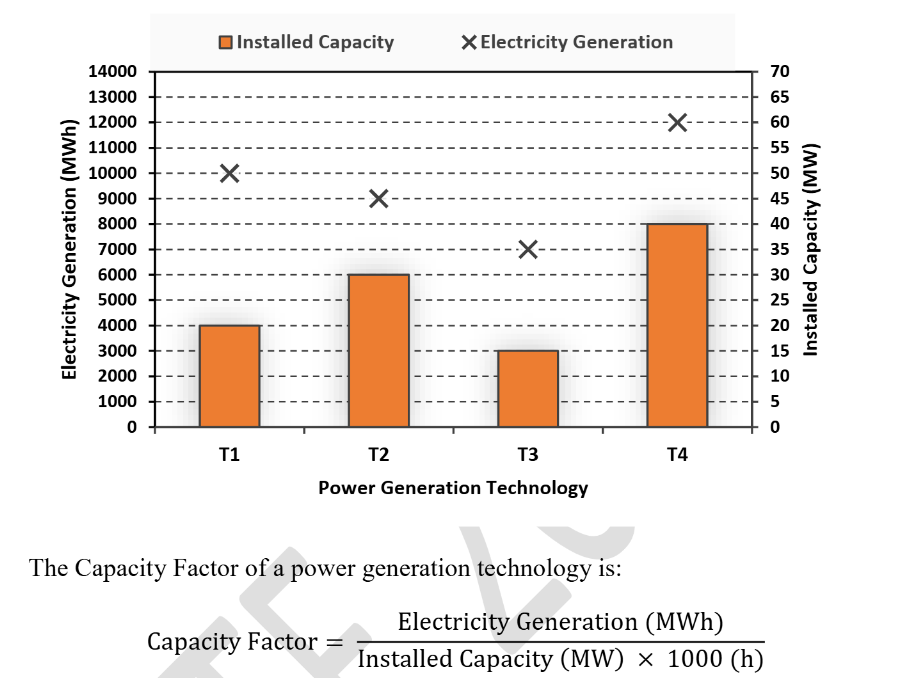
\includegraphics[width=0.4\textwidth]{figs/fig1.png}
    \caption{}
    \label{fig:q18}
\end{figure}


\hfill{\brak{\text{GATE GG 2024}}}

\begin{multicols}{4}
\begin{enumerate}
    \item T1
    \item T2
    \item T3
    \item T4
\end{enumerate}
\end{multicols}

\item In the $4 \times 4$ array shown below, each cell of the first three columns has either a cross (X) or a number, as per the given rule. Rule: The number in a cell represents the count of crosses around its immediate neighboring cells (left, right, top, bottom, diagonals). As per this rule, the maximum number of crosses possible in the empty column is
\begin{figure}[h!]
    \centering
    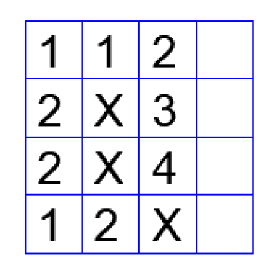
\includegraphics[width=0.4\textwidth]{figs/fig2.png}
    \caption{}
    \label{fig:q18}
\end{figure}


\hfill{\brak{\text{GATE GG 2024}}}

\begin{multicols}{4}
\begin{enumerate}
    \item 0
    \item 1
    \item 2
    \item 3
\end{enumerate}
\end{multicols}

\item During a half-moon phase, the Earth-Moon-Sun form a right triangle. If the Moon-Earth-Sun angle at this half-moon phase is measured to be $89.85^{\degree}$, the ratio of the Earth-Sun and Earth-Moon distances is closest to

\hfill{\brak{\text{GATE GG 2024}}}

\begin{multicols}{4}
\begin{enumerate}
    \item 328
    \item 382
    \item 238
    \item 283
\end{enumerate}
\end{multicols}

\textbf{PART A: COMPULSARY SECTION FOR ALL CANDIDATES}




\item The Earth's magnetic field originates from convection in which one of the following layers?

\hfill{\brak{\text{GATE GG 2024}}}

\begin{multicols}{2}
\begin{enumerate}
    \item Inner core
    \item Outer core
    \item Lithosphere
    \item Asthenosphere
\end{enumerate}
\end{multicols}

\item Which one of the following logging tools is used to measure the diameter of a borehole?

\hfill{\brak{\text{GATE GG 2024}}}

\item The given figure depicts an array used in DC resistivity surveys, where the current electrodes are denoted by C1 and C2, and potential electrodes by P1 and P2. If all the electrodes are equally spaced, then the given array corresponds to which one of the following configurations?
\begin{figure}[h!]
    \centering
    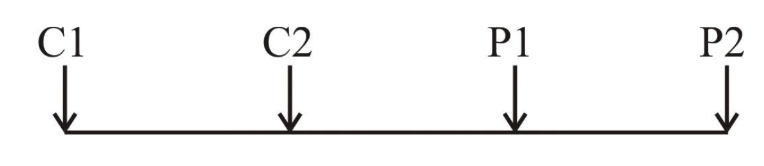
\includegraphics[width=0.4\textwidth]{figs/fig3.png}
    \caption{}
    \label{fig:q18}
\end{figure}


\hfill{\brak{\text{GATE GG 2024}}}

\begin{multicols}{2}
\begin{enumerate}
    \item Wenner
    \item Schlumberger
    \item Dipole-Dipole
    \item Pole-Pole
\end{enumerate}
\end{multicols}

\item Which one of the following is an ultramafic rock?

\hfill{\brak{\text{GATE GG 2024}}}

\begin{multicols}{4}
\begin{enumerate}
    \item Granite
    \item Gabbro
    \item Dunite
    \item Basalt
\end{enumerate}
\end{multicols}


\newpage

\item Gold is being produced from which one of the following mines in India?

\hfill{\brak{\text{GATE GG 2024}}}

\begin{multicols}{2}
\begin{enumerate}
    \item Baula
    \item Hutti
    \item Dariba
    \item Jaduguda
\end{enumerate}
\end{multicols}

\item Which of the following hydrocarbon fields is/are located in the western offshore of India?

\hfill{\brak{\text{GATE GG 2024}}}

\begin{multicols}{2}
\begin{enumerate}
    \item Tapti
    \item Lakwa
    \item Ravva
    \item Panna
\end{enumerate}
\end{multicols}

\item A cylindrical sample of granite \brak{\text{diameter = 54.7 mm; length = 137 mm}} shows a linear relationship between axial stress and axial strain under uniaxial compression up to the peak stress level at which the specimen fails. If the uniaxial compressive strength of this sample is 200 MPa and the axial strain corresponding to this peak stress is 0.005, the Young’s modulus of the sample in GPa is \underline{\hspace{1.5cm}} \brak{\text{in integer}}.

\hfill{\brak{\text{GATE GG 2024}}}




\item The given figure shows the ray path of a P–wave propagating through the Earth. Choose the CORRECT P–phase corresponding to the ray path.
\begin{figure}[h!]
    \centering
    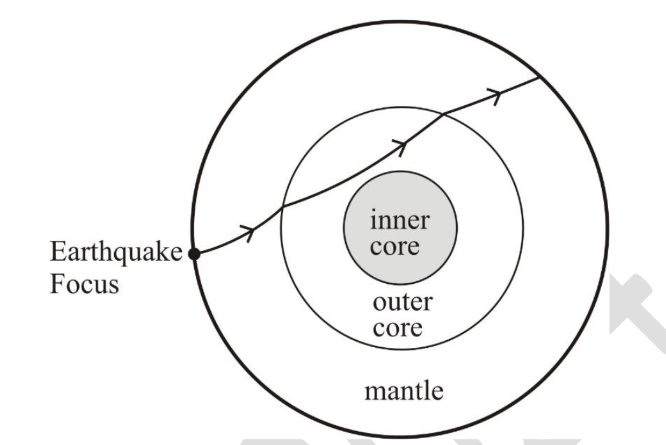
\includegraphics[width=0.4\textwidth]{figs/fig4.png}
    \caption{}
    \label{fig:q18}
\end{figure}


\hfill{\brak{\text{GATE GG 2024}}}

\begin{multicols}{4}
\begin{enumerate}
    \item PcP
    \item PKP
    \item PPP
    \item PmP
\end{enumerate}
\end{multicols}

\item Match the geophysical methods in Group–I with their associated physical properties in Group–II.
\begin{tabular}{ll}
\textbf{Group–I} & \textbf{Group–II} \\
P. Magnetic & 1. Chargeability \\
Q. Gravity & 2. Electrical conductivity \\
R. Magnetotelluric & 3. Susceptibility \\
S. Induced Polarization & 4. Density \\
\end{tabular}

\hfill{\brak{\text{GATE GG 2024}}}

\begin{enumerate}
    \item P-3, Q-4, R-2, S-1
    \item P-3, Q-4, R-1, S-2
    \item P-4, Q-3, R-2, S-1
    \item P-2, Q-1, R-4, S-3
\end{enumerate}
\newpage
\item The number of planes of symmetry in a tetrahedron is

\hfill{\brak{\text{GATE GG 2024}}}

\begin{multicols}{4}
\begin{enumerate}
    \item 9
    \item 6
    \item 4
    \item 3
\end{enumerate}
\end{multicols}


\item Which of the following Epochs belong(s) to the Quaternary Period?  

\hfill{\brak{\text{GATE GG 2024}}}

\begin{multicols}{2}
\begin{enumerate}
\item Holocene
\item Pleistocene
\item Pliocene
\item Miocene
\end{enumerate}
\end{multicols}

\item Which one or more of the following minerals shows O:Si ratio of 4:1 in its silicate structure?  

\hfill{\brak{\text{GATE GG 2024}}}

\begin{multicols}{2}
\begin{enumerate}
\item Olivine
\item Quartz
\item Diopside
\item Albite
\end{enumerate}
\end{multicols}

\item Which of the following rock structures is/are fold(s)?  

\hfill{\brak{\text{GATE GG 2024}}}

\begin{multicols}{2}
\begin{enumerate}
\item Antiform
\item Horst
\item Syncline
\item Synform
\end{enumerate}
\end{multicols}

\item Assume heat producing elements are uniformly distributed within a 16 km thick layer in the crust in a heat flow province. Given that the surface heat flow and reduced heat flow are 54 mW/m$^2$ and 22 mW/m$^2$, respectively, the radiogenic heat production in the given crustal layer in $\mu$W/m$^3$ is  (in integer).  

\hfill{\brak{\text{GATE GG 2024}}}

\item A confined aquifer with a uniform saturated thickness of 10 m has hydraulic conductivity of $10^{-2}$ cm/s. Considering a steady flow, the transmissivity of the aquifer in m$^2$/day is  (rounded off to one decimal place).  

\hfill{\brak{\text{GATE GG 2024}}}

\item A current of 2 A passes through a cylindrical rod with uniform cross-sectional area of 4 m$^2$ and resistivity of 100 $\Omega$-m. The magnitude of the electric field (E) measured along the length of the rod in V/m is  (in integer).  

\hfill{\brak{\text{GATE GG 2024}}}

\item Which one of the following lineations can be observed on a foliation with an attitude 210$^\degree$, 40$^\degree$ NW?  

\hfill{\brak{\text{GATE GG 2024}}}

\begin{multicols}{2}
\begin{enumerate}
\item 40$^\degree$ → 300$^\degree$
\item 40$^\degree$ → 040$^\degree$
\item 40$^\degree$ → 220$^\degree$
\item 40$^\degree$ → 350$^\degree$
\end{enumerate}
\end{multicols}

\item Match the minerals in Group–I with the corresponding cleavage types in Group–II.  

\begin{tabular}{p{0.48\textwidth} p{0.48\textwidth}}
\textbf{Group I} & \textbf{Group II} \\
P. Diopside & 1. Cubic \\
Q. Galena & 2. Octahedral \\
R. Calcite & 3. Prismatic  \\
S. Fluorite & 4. Rhombohedral \\
\end{tabular}  

\hfill{\brak{\text{GATE GG 2024}}}

\begin{multicols}{2}
\begin{enumerate}
\item P-3, Q-2, R-4, S-1
\item P-4, Q-3, R-1, S-2
\item P-3, Q-1, R-4, S-2
\item P-4, Q-1, R-2, S-3
\end{enumerate}
\end{multicols}



\item The composition of which one of the following reservoirs closely matches with that of iron meteorites?  

\hfill{\brak{\text{GATE GG 2024}}}

\begin{multicols}{2}
\begin{enumerate}
\item Primitive Mantle
\item Earth’s Core
\item Depleted Mantle
\item Bulk Silicate Earth
\end{enumerate}
\end{multicols}






\item Match the microstructures in Group–I with their characteristics in Group–II.  

\begin{tabular}{p{0.48\textwidth} p{0.48\textwidth}}
\textbf{Group I} & \textbf{Group II} \\
P.Core–mantle & 1.Radiating fibrous aggregate of K-feldspar
with or without quartz\\
 
Q. Decussate & 2. Large strained mineral grains surrounded
by fine-grained, recrystallized grains \\
R. Spherulite  & 3.Inclusion trails in a porphyroblast curves
into the matrix foliation by developing
concave outward pattern  \\
S. Millipede & 4. Randomly oriented mineral grains
dominated by crystal faces, such as in
sheet silicates\\
\end{tabular}

\hfill{\brak{\text{GATE GG 2024}}}

\begin{multicols}{2}
\begin{enumerate}
\item P-2, Q-3, R-4, S-1
\item P-3, Q-4, R-1, S-2
\item P-2, Q-4, R-1, S-3
\item P-4, Q-2, R-3, S-1
\end{enumerate}
\end{multicols}

\item Which one among the following is the least abundant sedimentary rock in the stratigraphic record?  

\hfill{\brak{\text{GATE GG 2024}}}

\begin{multicols}{2}
\begin{enumerate}
\item Sandstone
\item Limestone
\item Conglomerate
\item Shale
\end{enumerate}
\end{multicols}

\item Which one of the following sequences of index minerals correctly represents the order of increasing metamorphic grade during regional metamorphism of siliceous dolomitic limestones?  

\hfill{\brak{\text{GATE GG 2024}}}

\begin{multicols}{2}
\begin{enumerate}
\item Tremolite → Diopside → Talc
\item Diopside → Tremolite → Forsterite
\item Talc → Tremolite → Diopside
\item Talc → Forsterite → Tremolite
\end{enumerate}
\end{multicols}

\item Which one among the following is the oldest horse genus?  

\hfill{\brak{\text{GATE GG 2024}}}

\begin{multicols}{2}
\begin{enumerate}
\item Orohippus
\item Mesohippus
\item Merychippus
\item Pliohippus
\end{enumerate}
\end{multicols}

\item The measured plate velocity is maximum (in International Terrestrial Reference Frame) at which one of the following locations on the Indian Plate?  

\hfill{\brak{\text{GATE GG 2024}}}

\begin{multicols}{2}
\begin{enumerate}
\item Leh
\item Delhi
\item Bengaluru
\item Maldives
\end{enumerate}
\end{multicols}

\item Which one of the following textures is called the chalcopyrite disease?  

\hfill{\brak{\text{GATE GG 2024}}}

\begin{multicols}{2}
\begin{enumerate}
\item Chalcopyrite blebs in sphalerite
\item Sphalerite stars in chalcopyrite
\item Chalcopyrite lamellae in bornite
\item Bornite lamellae in chalcopyrite
\end{enumerate}
\end{multicols}

\item Which one of the following is the correct arrangement of volcanics from the oldest to the youngest?  

\hfill{\brak{\text{GATE GG 2024}}}

\begin{multicols}{2}
\begin{enumerate}
\item Bijli → Rajmahal → Malani → Deccan
\item Malani → Bijli → Deccan → Rajmahal
\item Bijli → Malani → Rajmahal → Deccan
\item Malani → Rajmahal → Bijli → Deccan
\end{enumerate}
\end{multicols}

\item Which of the following types of deposits is/are formed by fractional crystallization of magma?  

\hfill{\brak{\text{GATE GG 2024}}}

\begin{multicols}{2}
\begin{enumerate}
\item Komatiite hosted Ni–Cu
\item Peridotite hosted Cr
\item Leucogranite hosted U
\item Anorthosite hosted Ti–Fe
\end{enumerate}
\end{multicols}

\item Which of the following sedimentary basins is/are producing hydrocarbon commercially?  

\hfill{\brak{\text{GATE GG 2024}}}

\begin{multicols}{2}
\begin{enumerate}
\item Ganga
\item Krishna–Godavari
\item Kerala–Konkan
\item Cauvery
\end{enumerate}
\end{multicols}

\item Which of the following bivalves is/are swimmers?  

\hfill{\brak{\text{GATE GG 2024}}}

\begin{multicols}{2}
\begin{enumerate}
\item Aspergillum
\item Lima
\item Tellina
\item Pecten
\end{enumerate}
\end{multicols}

\item Which of the following structures is/are associated with duplexes in fold–thrust belts?  

\hfill{\brak{\text{GATE GG 2024}}}

\begin{multicols}{2}
\begin{enumerate}
\item Roof thrust
\item Floor thrust
\item Imbricate fan
\item Horses
\end{enumerate}
\end{multicols}




\item Which of the following statements is/are CORRECT ?  

\hfill{\brak{\text{GATE GG 2024}}}


\begin{enumerate}
\item Karst topography is formed in limestone terrains
\item Fjords are formed by aeolian activities
\item Oxbow lakes are formed in fluvial environments
\item Ventifacts are formed by glaciers
\end{enumerate}


\item Consider the solubility product of barite (BaSO$_4$) at 25 $^\circ$C and 1 bar to be $10^{-10}$. If the activities of Ba$^{2+}$ and SO$_4^{2-}$ ions are $0.5 \times 10^{-5}$ and $10^{-X}$, respectively, then the absolute value of `X` is  \brak{\text{rounded off to one decimal place}}.  

\hfill{\brak{\text{GATE GG 2024}}}

\item The support pressure of 20 kPa is required to stabilize the loose blocks of the Excavation Disturbed Zone (EDZ) at the crown of a circular tunnel with horizontal axis. The EDZ is to be stabilized by inserting rock bolts vertically into the roof. If the working capacity of a bolt is 160 kN, the area of the roof supported by a single bolt in m$^2$ is \brak{\text{in integer}}.  

\hfill{\brak{\text{GATE GG 2024}}}

\item The areas of drainage basins A and B are 25 km$^2$ and 50 km$^2$, respectively. The total length of drainages of all orders in basin A is 20 km. If both the basins have the same drainage density, the total length of drainages of all orders in basin B in km is \brak{\text{in integer}}.  

\hfill{\brak{\text{GATE GG 2024}}}

\item Match the stratigraphic units in Group--I with the sedimentary basins in Group--II.  

\begin{tabular}{p{0.48\textwidth} p{0.48\textwidth}}
\textbf{Group I} & \textbf{Group II} \\
P. Ramgundam Sandstone & 1. Chhattisgarh \\
Q. Raipur Formation & 2. Kaladgi\\
 
R. Bagalkot Group & 3. Marwar  \\
S. Sonia Sandstone& 4. Godavari \\
\end{tabular}   

\hfill{\brak{\text{GATE GG 2024}}}


\begin{enumerate}
\item P-2, Q-1, R-4, S-3
\item P-4, Q-1, R-2, S-3
\item P-4, Q-3, R-2, S-1
\item P-1, Q-4, R-3, S-2
\end{enumerate}


\item Which one of the following openings is a type of decline in underground mines?  

\hfill{\brak{\text{GATE GG 2024}}}

\begin{multicols}{4}
\begin{enumerate}
\item Crosscut
\item Winze
\item Spiral tunnel
\item Drift
\end{enumerate}
\end{multicols}

\item Which one of the following optic signs is CORRECT for a mineral with the given centered optic axis figure?  

\begin{figure}[h!]
    \centering
    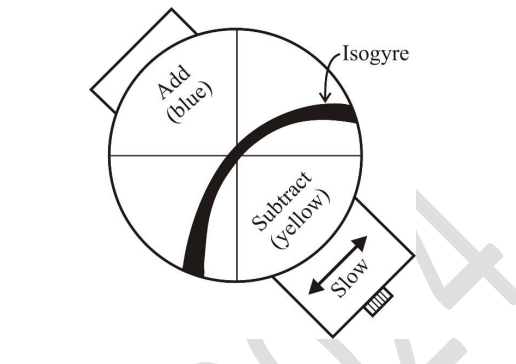
\includegraphics[width=0.4\textwidth]{figs/fig5.png}
    \caption{}
    \label{fig:q18}
\end{figure}



\hfill{\brak{\text{GATE GG 2024}}}

\begin{multicols}{4}
\begin{enumerate}
\item Uniaxial positive
\item Biaxial positive
\item Uniaxial negative
\item Biaxial negative
\end{enumerate}
\end{multicols}

\item Match the following invertebrates in Group--I with their morphological features in Group--II.  

\begin{tabular}{p{0.48\textwidth} p{0.48\textwidth}}
\textbf{Group I} & \textbf{Group II} \\
P. Trilobite & 1. Periproct \\
Q. Brachiopod & 2. Hypostome\\
 
R.Bivalve & 3. Deltidial plate  \\
S.Echinoid& 4. Lunule  \\
\end{tabular}   

\hfill{\brak{\text{GATE GG 2024}}}


\begin{enumerate}
\item P-2, Q-4, R-1, S-3
\item P-2, Q-3, R-4, S-1
\item P-4, Q-3, R-1, S-2
\item P-3, Q-2, R-4, S-1
\end{enumerate}


\item During high-temperature metamorphism of pelites, which one of the following mineral reactions represents the second sillimanite isograd?  

\hfill{\brak{\text{GATE GG 2024}}}


\begin{enumerate}
\item Muscovite + Quartz = Sillimanite + K-feldspar + H$_2$O
\item Staurolite + Quartz = Garnet + Sillimanite + H$_2$O
\item Staurolite + Muscovite + Quartz = Garnet + Biotite + Sillimanite + H$_2$O
\item Kyanite = Sillimanite
\end{enumerate}


\item Which one of the following represents deviatoric stress in a 2D stress Mohr Circle?  

\hfill{\brak{\text{GATE GG 2024}}}

\begin{multicols}{4}
\begin{enumerate}
\item Radius
\item Center
\item Pole
\item Diameter
\end{enumerate}
\end{multicols}

\item In the fold profile section shown in the figure, 1 and 3 are the oldest and the youngest stratigraphic units, respectively. Which one of the following fold descriptions CORRECTLY matches the asymmetric fold shown in the given figure?  

\begin{figure}[h!]
    \centering
    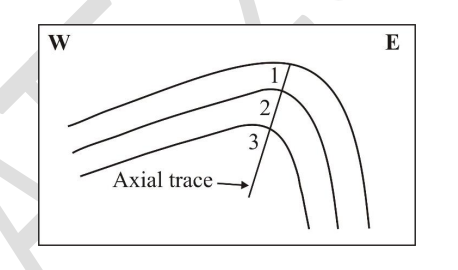
\includegraphics[width=0.4\textwidth]{figs/fig6.png}
    \caption{}
    \label{fig:q18}
\end{figure}


\hfill{\brak{\text{GATE GG 2024}}}

\begin{multicols}{2}
\begin{enumerate}
\item Antiform facing east
\item Synform facing east
\item Antiform facing west
\item Synform facing west
\end{enumerate}
\end{multicols}

\item If `X` represents the initial composition of a melt, which one of the trends indicated by arrows in the schematic diagram corresponds to the evolution of the residual melt composition during crystallization of diopside?  


\begin{figure}[h!]
    \centering
    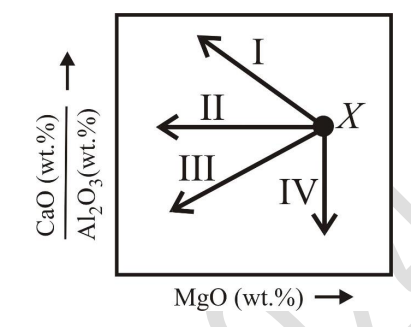
\includegraphics[width=0.4\textwidth]{figs/fig7.png}
    \caption{}
    \label{fig:q18}
\end{figure}

\hfill{\brak{\text{GATE GG 2024}}}

\begin{multicols}{4}
\begin{enumerate}
\item I
\item II
\item III
\item IV
\end{enumerate}
\end{multicols}

\item Match the following copper deposits in Group--I with their host rocks in Group--II.  

\begin{tabular}{p{0.48\textwidth} p{0.48\textwidth}}
\textbf{Group I} & \textbf{Group II} \\
P.Khetri & 1. Chlorite–biotite schist and soda–granite \\
Q. Mosabani  & 2. Garnetiferous chlorite schist\\
 
R.Malanjkhand & 3. Metachert  \\
S.Kalyadi& 4.Tonalite–granodiorite–granite  \\
\end{tabular}  
\hfill{\brak{\text{GATE GG 2024}}}

\begin{enumerate}
\item P-2, Q-3, R-4, S-1
\item P-4, Q-1, R-2, S-3
\item P-2, Q-1, R-4, S-3
\item P-3, Q-4, R-1, S-2
\end{enumerate}


\item Which one of the following events represents the termination of the Wilson Cycle in Plate Tectonics?  

\hfill{\brak{\text{GATE GG 2024}}}


\begin{enumerate}
\item Ocean--continent subduction
\item Continent--continent collision
\item Continental rifting
\item Seafloor spreading
\end{enumerate}

\item The fraction of the incident electromagnetic energy reflected from a material is known as  

\hfill{\brak{\text{GATE GG 2024}}}

\begin{multicols}{4}
\begin{enumerate}
\item acuity
\item albedo
\item spectral hue
\item artifact
\end{enumerate}
\end{multicols}

\item Which of the following statements regarding ore deposits is/are CORRECT ?  

\hfill{\brak{\text{GATE GG 2024}}}


\begin{enumerate}
\item Both replacement and exhalative ores are possible in SEDEX type deposits
\item Rampura--Agucha Pb--Zn deposit is a Mississippi Valley Type deposit
\item Orogenic gold deposit is an epigenetic type deposit
\item Fluid boiling in the early stage of magmatic crystallization is responsible for Cu--(Mo) deposits
\end{enumerate}


\item Which of the following sedimentary structures is/are found in intertidal deposits?  

\hfill{\brak{\text{GATE GG 2024}}}

\begin{multicols}{2}
\begin{enumerate}
\item Ladder-back ripple
\item Rain print
\item Double mud drape
\item Mud-crack
\end{enumerate}
\end{multicols}

\item Which of the following materials is/are used for estimation of hydrocarbon source rock maturation based on color?  

\hfill{\brak{\text{GATE GG 2024}}}

\begin{multicols}{2}
\begin{enumerate}
\item Conodont
\item Illite
\item Spore
\item Zircon
\end{enumerate}
\end{multicols}

\item Which of the following schist belts occur(s) to the east of the Closepet Granite in southern India?  

\hfill{\brak{\text{GATE GG 2024}}}

\begin{multicols}{2}
\begin{enumerate}
\item Shimoga
\item Kolar
\item Bababudan
\item Hutti
\end{enumerate}
\end{multicols}

\item The diagram given below shows phase relations between components P and Q at 1 bar pressure. If `X` represents the initial liquid composition, which of the following statements is/are CORRECT during equilibrium crystallization?  

\begin{figure}[h!]
    \centering
    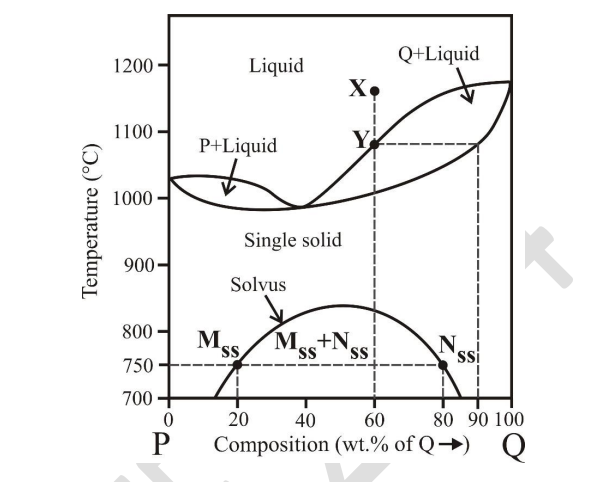
\includegraphics[width=0.4\textwidth]{figs/fig8.png}
    \caption{}
    \label{fig:q18}
\end{figure}


\hfill{\brak{\text{GATE GG 2024}}}


\begin{enumerate}
\item Initial liquid composition is 60 wt.\% of P and 40 wt.\% of Q
\item The composition of the solid in equilibrium with the liquid at `Y` is 10 wt.\% of P and 90 wt.\% of Q
\item The bulk composition of the final solid product is 40 wt.\% of P and 60 wt.\% of Q
\item The proportion \brak{\text{on the basis of wt.\%}} of two phases, MSS : NSS is 1 : 2 at 750 $^\circ$C
\end{enumerate}


\item Which of the following statements is/are CORRECT for the M-plane of any fault?  

\hfill{\brak{\text{GATE GG 2024}}}


\begin{enumerate}
\item M-plane pole of a fault is located on the fault plane
\item M-plane pole of a fault is perpendicular to the slickenline on the fault plane
\item M-plane pole of a fault is parallel to the slickenline on the fault plane
\item M-plane pole of a fault is perpendicular to the pole to the fault plane
\end{enumerate}


\item Which of the following microfossils is/are foraminifera?  

\hfill{\brak{\text{GATE GG 2024}}}

\begin{multicols}{2}
\begin{enumerate}
\item Miliammina
\item Triceratium
\item Cibicides
\item Guembelitria
\end{enumerate}
\end{multicols}

\item The in situ stress at a point in a dry sandstone terrain is as follows: $\sigma_1 = 12$ MPa and $\sigma_3 = 4$ MPa. The pore water pressure ($p_w$) increases by the construction of a reservoir. The failure criterion of the sandstone is given by  $\sigma_1^{\prime} = 3.48$ MPa $+ 3\,\sigma_3^{\prime}$, where $\sigma_1^{\prime}$ and $\sigma_3^{\prime}$ are the effective maximum and minimum principal stresses, respectively. Assuming that the failure occurs at peak stress, the minimum value of $p_w$ \brak{\text{in MPa}} that will cause the sandstone to fail in situ is  \brak{\text{rounded off to two decimal places}}.  

\hfill{\brak{\text{GATE GG 2024}}}

\item If the Rb--Sr isochron formed by a suite of gabbro samples has a slope of 0.0265, then the calculated age of the gabbro in million years is $\lambda(^{87}\mathrm{Rb})=1.42\times10^{-11}$ year$^{-1}$}}  

\hfill{\brak{\text{GATE GG 2024}}}

\item A soil mass comprises two horizontal layers \brak{\text{of equal thickness and equal width}} stacked one above the other. The hydraulic conductivities of the two layers are $5 \times 10^{-2}$ cm/s and $3 \times 10^{-2}$ cm/s. Considering Darcian flow of water and same hydraulic gradient for both the layers, the effective hydraulic conductivity of the soil mass in cm/s is \brak{\text{rounded off to two decimal places}}.  

\hfill{\brak{\text{GATE GG 2024}}}








\end{enumerate}

\begin{align*}
 {\LARGE{\textbf{END OF THE QUESTION PAPER}}}
\end{align*}





\end{document}